Full documentation for \texttt{GraphEvolve.jl} can be found at \href{https://percolation.fun}{https://percolation.fun}.

\section{Designing the Library}
I chose Julia as the language to write the library in for several reasons, the largest being that I believe Julia is the perfect language for running large scale distributed computational physics/mathematics simulations.
The benefit of being able to use it as an interactive language while at the same time getting speeds of a compiled language can not be understated since the immediate feedback and ability keep a kernel running with data in RAM allows for easy debugging and data exploration.
Julia code revolves around its type system which works nicely with its use of multiple dispatch, and at the heart of the type system is defining custom types and creating hierarchies with which functions can take specific types.
The type hierarchy of Julia's default types is illustrated in Fig. \ref{fig:julia_type_hierarchy}.

\begin{figure}[H]
	\centering
	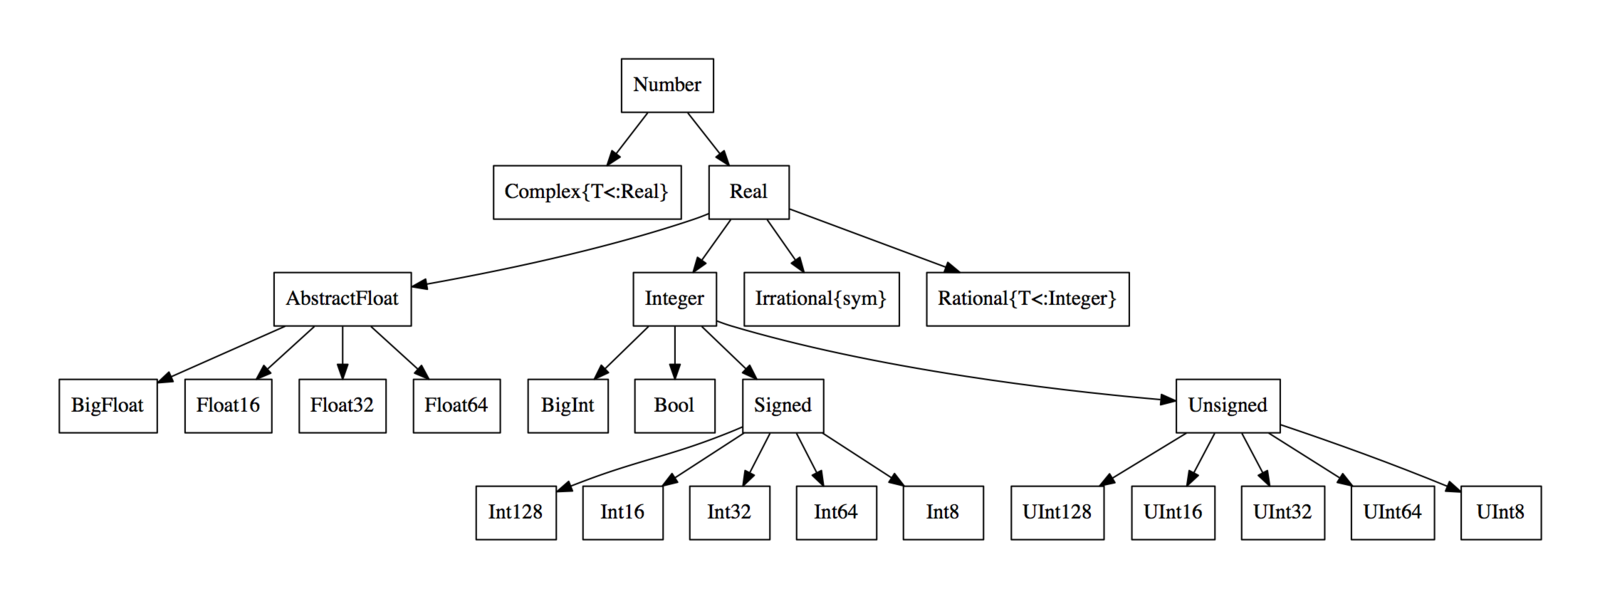
\includegraphics[width=400pt]{images/julia_type_hierarchy.png}
	\caption{Julia Type Hierarchy}
	\label{fig:julia_type_hierarchy}
\end{figure}

The type system is actually opt-in, meaning that one need not type their variables, but typing can help with performance as well as gaining a better understanding of how the code works.

I started off with creating custom types to represent networks/lattices, the type hierarchy of them is illustrated below in Fig. \ref{fig:custom_type_hierarchy}.

\begin{figure}[H]
	\centering
	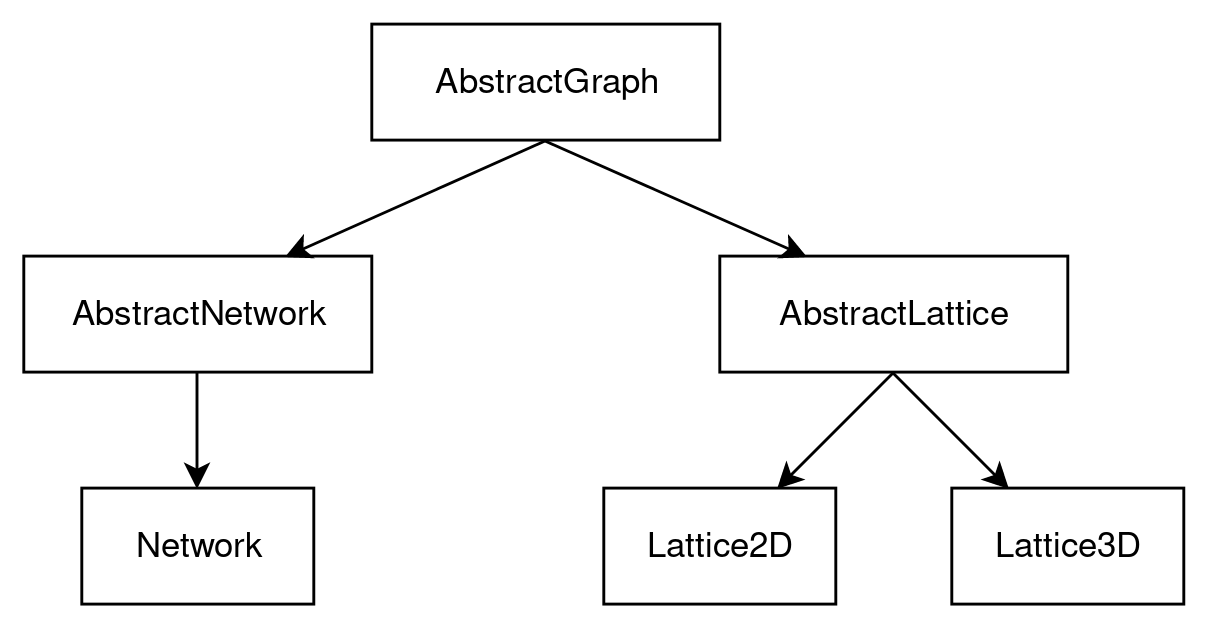
\includegraphics[width=350pt]{images/custom_type_hierarchy.png}
	\caption{Custom Type Hierarchy}
	\label{fig:custom_type_hierarchy}
\end{figure}

As of now there are three different types of graphs: \texttt{Network}, \texttt{Lattice2D}, and \texttt{Lattice3D}.
The \texttt{Network} type represents an undirected random network where edges can be present between any two unique nodes.
The \texttt{Lattice2D} type represents a two-dimensional square lattice where edges can be present only between nearest neighbors, similarly where \texttt{Lattice3D} represents a three-dimensional cubic lattice.
The following is a brief conceptual overview of how the system functions, for more detailed descriptions and explanations of methods or variables please refer to the documentation.

Each of these types have a similar structure in the way they store information about the underlying graph they represent.
To instantiate a type one must pass it the system size and optionally a seed value for the random number generator (which is used in the evolution for randomly selecting edges), which in a \texttt{Network} means passing the number of nodes \texttt{n} and in a \texttt{LatticedD} passing the side length \texttt{L} ($\texttt{n} = \texttt{L}^\texttt{d}$).
The types also have a variable called \texttt{t} which refers to the step in the evolution process and represents the number of edges present in the graph.
The edges present in the graph are kept track in the \texttt{edges} variable, which is a set of two-tuples of integers representing an edge between node \texttt{i} and \texttt{j} as \texttt{(i, j)}.
As of now the edges in all types are undirected i.e. \texttt{(i, j) = (j, i)}, but only \texttt{(i, j)} is stored to minimize unnecessary RAM usage.

Keeping track of the clusters as they evolve is the meat of these simulations, therefore it is necessary to speak about how this is done.
\texttt{cluster\_ids} is a \texttt{d}-dimensional array \texttt{(d = 1 (Network), 2 (Lattice2D), 3 (Lattice3D))} which contains the information relating to which cluster a node is in.
\texttt{clusters} is a dictionary where the keys are the cluster IDs and the values are sets of nodes which are in the given cluster.
\texttt{cluster\_sizes} is a dictionary where the the keys are the cluster sizes ($s$) and the values are the cluster counts ($n_s$).
The associated observables are stored in a custom type called \texttt{Observables} under the name \texttt{observables}.

Now that we understand how the clusters are tracked let's talk about how this is done in reality.
Let \texttt{t} be the current step in the evolution process where edge \texttt{(i, j)} has been chosen to be added to the graph.
Let $C_\texttt{i}$ represent the cluster to which node \texttt{i} is a member of, i.e. $\texttt{i} \in C_\texttt{i}$.
We then look and determine which cluster is smaller and merge the smaller cluster into the larger cluster in-place (this small trick saves a significant amount of computational time), e.g. if $|C_\texttt{j}| < |C_\texttt{i}|$ then all of the nodes in $C_\texttt{j}$ will have their cluster ID updated to that of $C_\texttt{i}$ and the set of nodes representing $C_\texttt{i}$ will be updated to include the nodes in $C_\texttt{j}$, and the entry for $C_\texttt{j}$ will then be deleted from \texttt{clusters} to reduce the memory footprint.

After the clusters are merged the associated observables are updated, which currently includes the largest cluster size, the average cluster size, the cluster heterogeneity (number of unique cluster sizes), and some post-simulation analysis quantities used for identifying where the phase transitions and if it is continuous.



\subsection{Making Use of Multiple Dispatch}
Multiple dispatch allows us to define multiple functions with the same name, yet different code depending on the input type.
This is extremely useful for dealing with differences between networks and lattices such as when selecting an edge, because for example in a \texttt{Network} we can select any inactive edge between nodes, whereas in a \texttt{LatticedD} we can only select an inactive edge between nearest neighbors (this can be seen implemented in \texttt{edge\_methods.jl}).

Another benefit of this coupled with the type system is that when we have a function that is generic enough to act on both \texttt{Network}s and \texttt{LatticedD}s then we can set the input type for that function to \texttt{AbstractGraph} or if it's general enough to act on all \texttt{LatticedD}s but not \texttt{Network}s then we can set the input type to \texttt{AbstractLattice}.
This allows for consistency, e.g. we can call \texttt{product\_rule!(Network(Int(1e6)))} and similarly\\\noindent \texttt{product\_rule!(Lattice2D(Int(1e3)))} and the code will decide based on the type which functions to use.



\subsection{Making Use of Parallelization}
Currently when a single simulation is run it is run on a single core.
For the data used in this thesis I use a script which has a parallel for loop which takes advantage of all threads that are enabled to run simulations in parallel with different seed values.
Recently the Julia developers published an article talking about "composable multi-threaded parallelism", which is currently in the early stages, but looks promising and could make future parallelization very easy.
Once stable it can be implemented in \texttt{GraphEvolve.jl} to run the updating of the observables in a separate thread, i.e. if we would like to gather information about an observable that takes too much time to run on the single thread we could spawn a new thread to compute this in parallel with the rest of the simulation.



\subsection{Running a Simulation}
Running a simulation is simple, one must first download the \texttt{GraphEvolve.jl} library, which can be found on GitHub under the MIT license.
Then, to run a simulation on a \texttt{Network} with $10^6$ nodes using the product rule to add $1.5 \cdot 10^6$ edges, and view the largest cluster size time series data we would run:

\begin{lstlisting}
julia> using GraphEvolve

julia> using Plots; pyplot(fmt="png"); using LaTeXStrings

julia> PyPlot.matplotlib.rc("mathtext", fontset="cm");

julia> PyPlot.matplotlib.rc("text", usetex=true);

julia> PyPlot.matplotlib.rc("font", family="serif", size=12);

julia> g = Network(10^6);

julia> stochastic_edge_acceptance!(g, Int(1.5*10^6));

julia> x = collect(0:g.t) ./ g.N;

julia> y = g.observables.largest_cluster_size ./ g.N;

julia> plot_ = plot(dpi=300);

julia> scatter!(x, y,
           legend=false,
           marker=(2, :dodgerblue, :circle, 0.9, stroke(0)),
           xaxis=(latexstring("t/N"), (0, 1.5), 0:0.5:1.5),
           yaxis=(latexstring("|C|/N"), (0, 1), 0:0.2:1)
       );

julia> savefig(plot_, "/tmp/order_param.png")
\end{lstlisting}
